In this paper, we will center our attention on a class of decision problems
corresponding to the following formalism. There exists some population of 
individuals $I = \{i_1, i_2, \ldots, i_n\}$ over whom we must distribute some
resource $R$. A \textit{decision rule} is a mapping $d \rightarrow \{0, 1\}$,
under which $i_n$ receives $R$ iff $d(i_n) = 1$. As an example, consider the
process of allocating loans over a pool of applicants — for each individual in
the applicant pool, we have a binary choice to either approve or deny the loan,
and only on acceptance does the individual receive capital.

An algorithmic decision maker in this setup is a system, particularly a
technical system, under which a decision rule is implemented as a set of steps
which are applied identically to all individuals. This broadly consists of two
tasks. First, a set of covariates $X$ must be collected for each individual.
Then, a classification scheme $f: X \rightarrow \{0, 1\}$ must be used to map
each individual to an outcome. Returning to the loan case, a simple example
would be the following: Approve a loan to each individual whose household
income exceeds the projected cost of living in the geographic location of their 
esidence by at least \$10,000 per year. Then our algorithm implementing the
decision rule for each applicant takes the following shape:
\begin{itemize}
    \item Collect covariates $X=\{$household income, goegraphic location of residence$\}$
    \item Let $C =$ projected cost of living in location of residence, $H =$
          household income
    \item $f = H - C \geq 10000$
\end{itemize}

It is important to note that not all problem domains to which algorithmic
decision making is applied can be formulated in this way. For example,
applications of AI in natural language translation may not be easily formulated
in terms of resource allocation, but the reader may still be concerned with the
perpetuation of social biases through the decisions made in translation — for
example, issues of underrepresentation of social groups in translated media.  
While these cases are significant, they do not fall simply within the domain of
distributive justice, and so will not be considered here.

\subsection{Algorithmic Fairness Measures}\label{sec:fairness-measures}

Algorithmic fairness measures as they're presented in the literature operate on
the classification scheme $f$ and a set of morally protected characteristics
such as race or gender $A \subseteq X$, attempting to enforce contraints on how 
decisions can be sensitive to such characteristics. An overview of measures
commonly discussed in the literature is presented below.

\todo{Elaborate/improve discussion of individual/group}
A critical point to note in the discussion of algorithmic fairness is the 
distinction between individual and group fairness. Individual fairness
focuses on the fair treatment of a single individual, while group fairness
focuses on the fair treatment of groups of people identified by some common
morally protected characteristic. A typical approach to individual fairness is
to require that similar individuals be treated similarly, while group fairness
requires balancing statistical quantiites of outcomes across groups. For our
purposes, both individual and group fairness can be characterized by what
constraint they pose on the classification function, and so we will be able to
analyze both through the same lens of distributive justice.

As a running example, consider the case of a hiring algorithm. The decision
problem is to map a set of applicants to hiring decision. Our algorithm must
implement a function to do so based only on the personal information presented
in their resumes, which is their education, experience, and cover letter. We
want to ensure that our hiring practices are fair with respect to race, and
gender. This gives us the following setup:

\todo{Rework Figure}

\begin{center}
    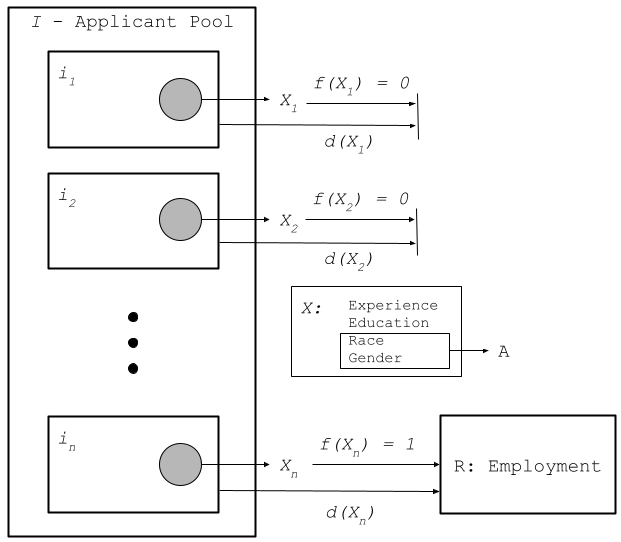
\includegraphics[scale=.4]{figs/fig1.png}\\
    \emph{Fig. 1: A hiring decision algorithm as a decision problem}\\
\end{center}
where a fairness measure will operate exclusively on the mapping from
experience, education, cover letter, race, and gender to hiring decisions.

Some of the most commonly discussed measures in the literature are presented
below together with their strengths critiques leveraging this lens. For a more
exhaustive list of measures, see~\cite{CorbettDavies_2023}.

\todo{Revise definitions}

\begin{definition}
    Fairness Through Unawarenss — $f$ satisfies fairness through unawareness iff
    \[A = \emptyset\]
\end{definition}

In other words, the classification function may not receive any morally
protected covariates as inputs. So, for our hiring admissions case, we would be
forced to remove race and gender from $X$ and only consider education and
experience.

This notion is intuitively appealing — how can the algorithm dicriminate against
me based on my race if it doesn't know my race? However, it is clear that this
measure is not sufficient to ensure fairness. For example, if one attended a
historically black college, their education may function as a proxy for their
race, allowing bias to remain in the algorithm.

\begin{definition}
    Demographic Parity — $f$ satisfies demographic parity iff
    \[P[f(X) = 1 | A = a] = P[f(X) = 1]\;\forall a \in A\]~\citep{Dwork_2012}.
\end{definition}

Demographic parity holds that the probability of a positive output ($f(X) = 1$)
should be statistically independent of the protected attributes. This is 
an easily understandable and measurable criteria for fairness. At a first look,
it is appealing — the same number of individuals from each race will be
successful in seeking jobs at a particular company. However, a close look
reveals difficulties.

Under demographic parity, we must balance the probability of success between
groups, which becomes very difficult when the base rates of success are
unequal. For example, if women are much more qualified for a job on average than
men, then demographic parity will require that we hire less qualified men in
place of more qualified women in order to balance the probability of being selected
between gender groups. In other words, my false positive rate will be very high
for men while my false negative rate will be very high for women, creating a 
severely unfair practice~\citep{Barocas_2017}.

\begin{definition}
    Equalized Odds — $f$ satisfies equalized odds if given true outcomes $D$
    over all individuals, we have
    \[P[Y=1|A=a, D=1] = P[Y=1|A=b, D=1]\;\forall a, b\in A\]
    \[P[Y=1|A=a, D=0] = P[Y=1|A=b, D=0]\;\forall a, b\in A\]~\citep{Hardt_2016}.
\end{definition}

Equalized odds requires that the true positive and false positive rates be
balanced between groups. This is often thought to ensure there is no disparate 
mistreatment across groups. In our hiring case, for example, equalized odds
ensures that no one racial group is more likely to be falsely rejected or
erroneously hired than another. Given one has been rejected, the probability it
was a wrongful rejection is equal regardless of their race or gender.

Equalized odds is often critiqued for struggling to deal with unequal base rates
between groups. Consider the following example from criminal justice. We have a 
distribution rule which says to allocate a parole to a prisoner if they are very
unlikely to recidivate. Due to a history of discriminatory practices and social
marginalization, black prisoners have a base rate of recidivism much higher than
white defendants~\citep{CrimeJustice_2023}. As a result, allocating a parole to 
a white prisoner has a base line lower likelihood of being a false positive. 
Therefore, one could achieve equal false positive rates by \textit{adding} false
positives to the white portion of the dataset, resulting in an increase in the
number of white prisoners receiving parole undeservingly. 

As an example of equalized odds gone wrong, consider the COMPAS
algorithm~\citep{Angwin_2016}. COMPAS was calibrated to have equal predictive
accuracy across racial groups, but this resulted in a higher false positive rate
for black defendants and a much lower false positive rate for white defendants
due to unequal base rates.

\begin{definition}
    Counterfactual Fairness — $f$ satisfies counterfactual fairness iff
    \[P[f_{A \leftarrow a}(X) = 1 | X = x, A = a] = P[f_{A\leftarrow b}(X) = 1 |
         X = x, A = a]\;\forall a, b \in A\]~\citep{Kusner_2018}.
    Where $P(f_{A \leftarrow a})$ is the counterfactual value of $f$ if $A$ were
    set to $a$.
\end{definition}

Borrowing from the language of causal inference, counterfactual fairness posits
that the protected attributes may not have any causal effect on the outcome of
the classification function. Holding the other covariates constant, if we were to
change the value of a protected attribute, the outcome of the classification
function should not change. This is a highly appealing notion of fairness.
If their protected characteristics do not in any way cause their outcome, then
it is difficult to argue that one has been discriminated against. However,
this measure is difficult to implement in practice.

Counterfactual fairness is often critiqued based on the difficulty and potential
subjectivity of detecting causal links between variables. Recent work on the 
social construction of demographic variables reveals that causal modeling may 
have an inherently normative basis~\citep{Hu_Forthcoming}, and even if these
issues are set aside, the computational expense of causal discovery can create
issues of practicality.

This discussion of dominant algorithmic fairness measures and their critiques
reveal that there is no one-size-fits-all solution to the problem of algorithmic
fairness. Each measure has its own strengths and weaknesses, and the choice of
measure will depend on the specific context in which the algorithm is being
applied. However, how should one select a measure? What are the normative
considerations that should guide this choice? In hopes of developing a more
nuanced and structured approach to these questions, we turn to work in the 
philosophy of distributive justice.

\subsection{Theories of Distributive Justice}

Distributive justice is a philosophical field of inquiry that examines how to
define a fair allocation of goods and resources across a society. A fully
fledged account of distributive justice must answer a number of questions. Who
should receive those resources which are highly scarce? When and why is it 
allowed for one person to have more of something than another? By what mechanism
can resources be redistributed to achieve justice?

Given that distributive justice defines how fair decisions about allocations can
be made, within the formalism we've presented, its role is to broadly define the
decision rule which may then be implemented algorithmically. As described in
section~\ref{sec:introduction}, the dominant theory of distributive justice used
in connection with algorithmic decision making is John Rawls' theory of liberal
egalitarianism, which we will present here.

Rawls introduces his account of justice through a thought experiment called the
veil of ignorance. In this experiment, one is asked to imagine themselves in a
pre-societal world, working in collaboration with a number of others to
determine how resources should be allocated across society once it begins. 
Criticaly, all those involved in designing this distribution of goods are
unaware of what their own position and endowments in society will be. One may
find themself endowed with a high level of intelligence, or a valuable skill, or
wealth at birth, or one may find themself with none of these things, or the
opposite. Without knowing which of these positions one will occupy, Rawls argues
that one will be motivated to design a society in which the following two
principles are satisfied:

\begin{enumerate}
    \item Each person has an indefeasible right to the most extensive basic 
          liberties compatible with equal liberty for all.
    \item Social and economic inequalities are to be arranged so that they are
          both to the greatest benefit of the least advantaged, to offices
          open under fair equality of opportunity. (dubbed the
          \textit{difference principle}).
\end{enumerate}

Rawls refers to the group of individuals designing the society from behind the
veil of ignorance as the \textit{original position}. The argument from the
original position results in citizens living under a social contract which
is guided by the two principles given above. The principles allow us to measure,
for any given distribution of resources across society, whether or not the
distribution is fair. If the distribution is not fair, then Rawls endorses
a program of redistribution to bring the distribution into line with the
principles. For example, a soicety with a high-level of wealth inequality is
in violation of the difference principle — the wealth gap represents an economic
inequality which is not to the greatest benefit of the least advantaged. In this
case, Rawls would endorse a program of redistribution to balance the wealth
across the society in accord with the principles given above.

This type of distributive justice theory is what we refer to as an
\textit{end-state} theory of justice. The distribution of goods across society
represents a discretely evolving state of affairs, and the role of the theory is
to determine whether or not each state is just. Let us consider this view in
light of the decision problem we formalised above. Liberal egalitarianism tells
us that the decision rule $d$ must be such that either all individuals receive
the resource of allocation equally, or that inequalities in the allocation of
resources must be to the benefit of the least advantaged. Several of the
fairness criteria in the literature on algorithmic fairness can be seen as
implementing the first condition in terms of equality of opportunity — by 
regulating the extent and manner in which protected attributes can influence the
outcome of the decision, we attempt to ensure that all individuals are entitled
to equal basic rights of opportunity in the decision process. However, whether
or not the difference principle is satisfied by these measures is less clear.

In our load case, for example, we may be concerned with ensuring that every
individual receives equal opportunity to a loan. However, if the decision rule
is such that only individuals with a household income above \$100,000 per year,
or those who are members of a particular race, are able to receive a loan, then
this clearly doesn't provide equal opportunity to all. A measure like
demographic parity ensures that individuals from each protected group is equally
likely to receive a loan, therefore balancing opportunity across groups. However,
whether or not this satisfies the difference principle depends on the base rates
of success across groups. If the base rate of loan default is higher for men
than for women, demographic parity may require that we give loans to some men
who are less likely to pay back their loans rather than qualified women, and in
doing so, we are certainly not distributing inequalities to the less advantaged
as we would need to under the difference principle.
